\section{Empirical Evaluation}
In this section, we evaluate our approach and test three
hypotheses: First, does incorporating model-based priors help speed up
the convergence of {\sc maxq} to the optimal policy? Second, since in
this case both the prior and the structure of the task hierarchy
convey information about the structure of the task, how do they
interact? Does the task hierarchy still matter if very good priors are
available for primitive actions? Finally, how does Bayesian HRL
compare to standard (flat) Bayesian RL? Does Bayesian RL perform
better (in terms of computational time) if a task hierarchy is available?

\begin{figure*}[ht]
\begin{tabular}{cc}
\hspace{-1in}\includegraphics[scale=0.6]{Taxi-Hierarchy.pdf} &
\hspace{-2.5in}\includegraphics[scale=0.6]{Wargus-Hierarchy.pdf}\\
\vspace{-5.2in}
\end{tabular}
\caption{Task Hierarchies for {\sf Taxi-world} (left) and {\sf Resource-collection} (right).}\label{fig:tasks}
\end{figure*}

\begin{figure*}[t]
\centerline{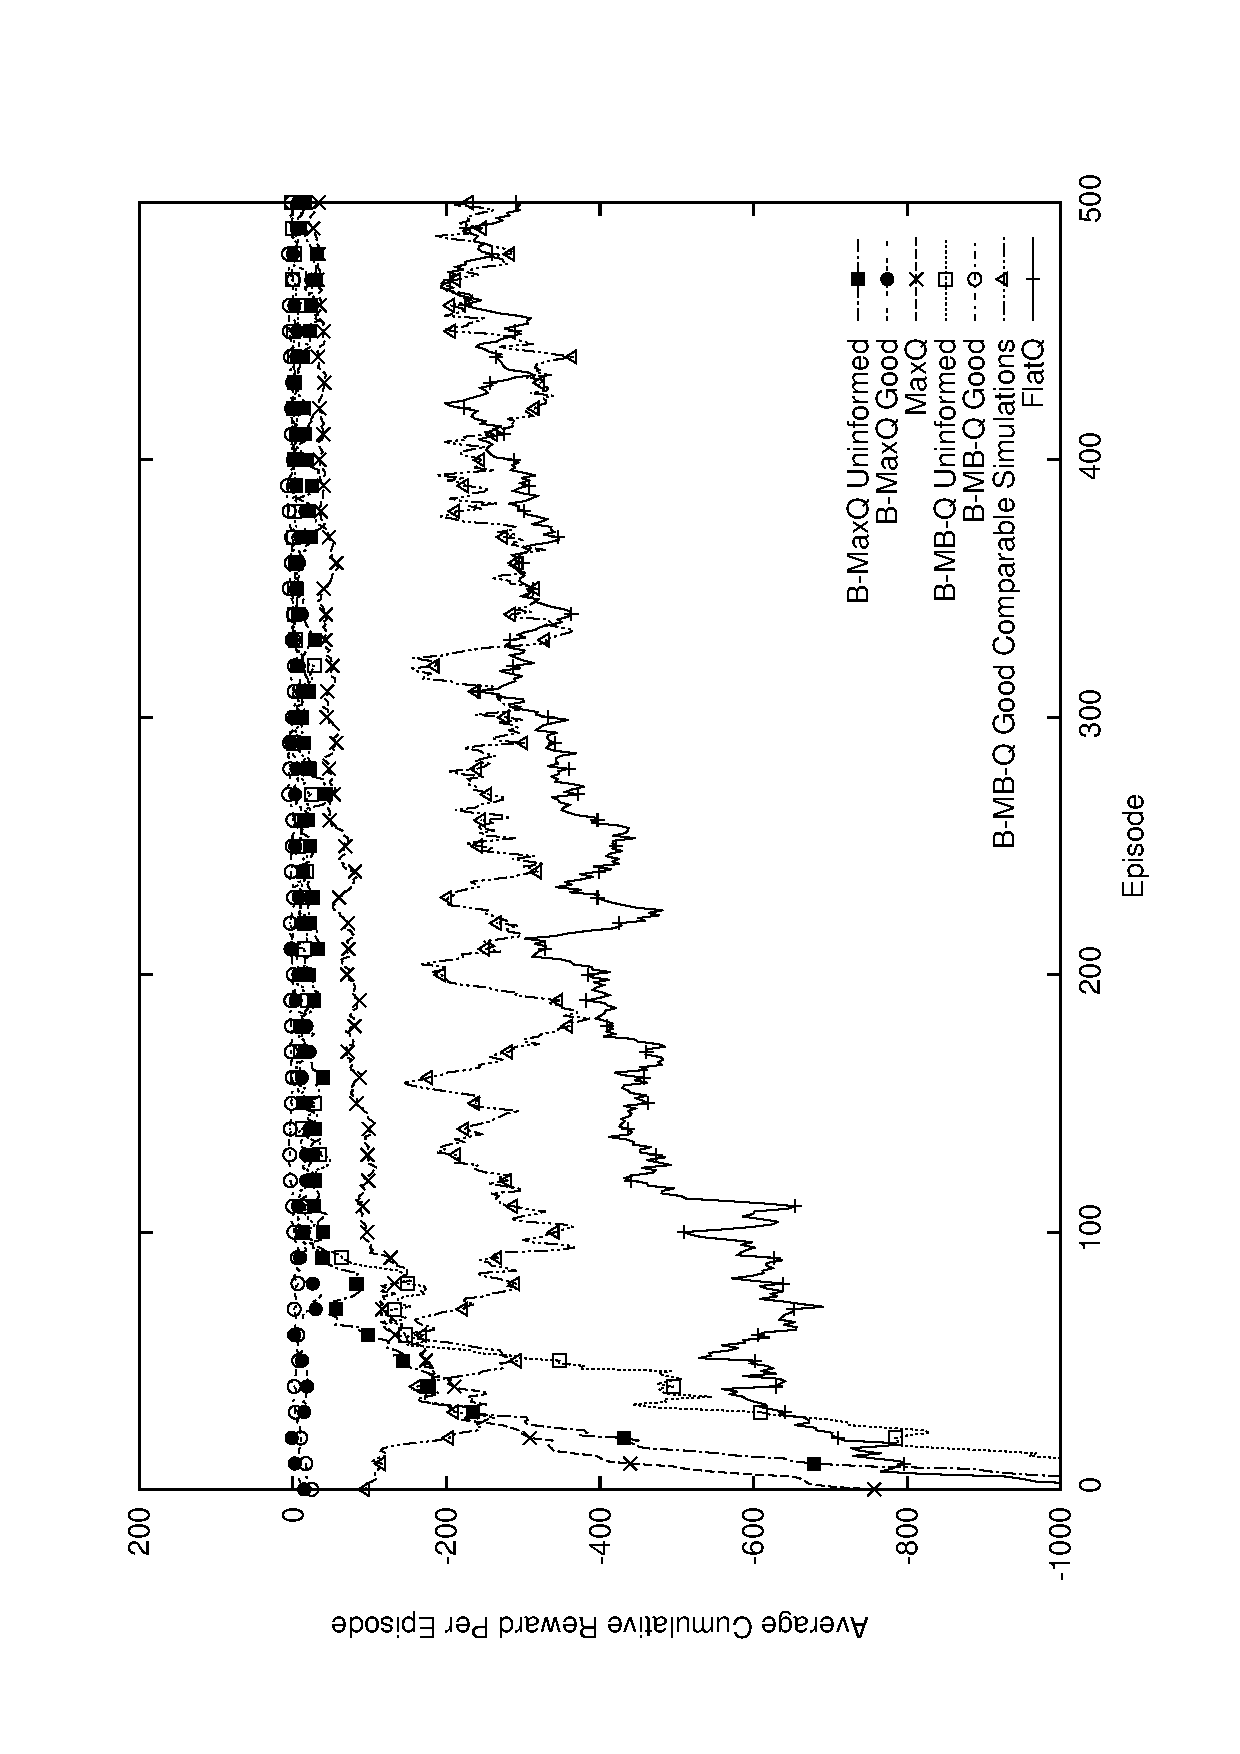
\includegraphics[scale=0.4]{Taxi.pdf}}
\vspace{-0.5in}
\caption{Performance of different algorithms on {\sf Taxi-world}. The
  prefix ``B-'' denotes Bayesian, ``Uninformed/Good'' denotes the
  prior and ``MB'' denotes model-based.}\label{fig:taxi}
\end{figure*}
\begin{figure*}[t]
\centerline{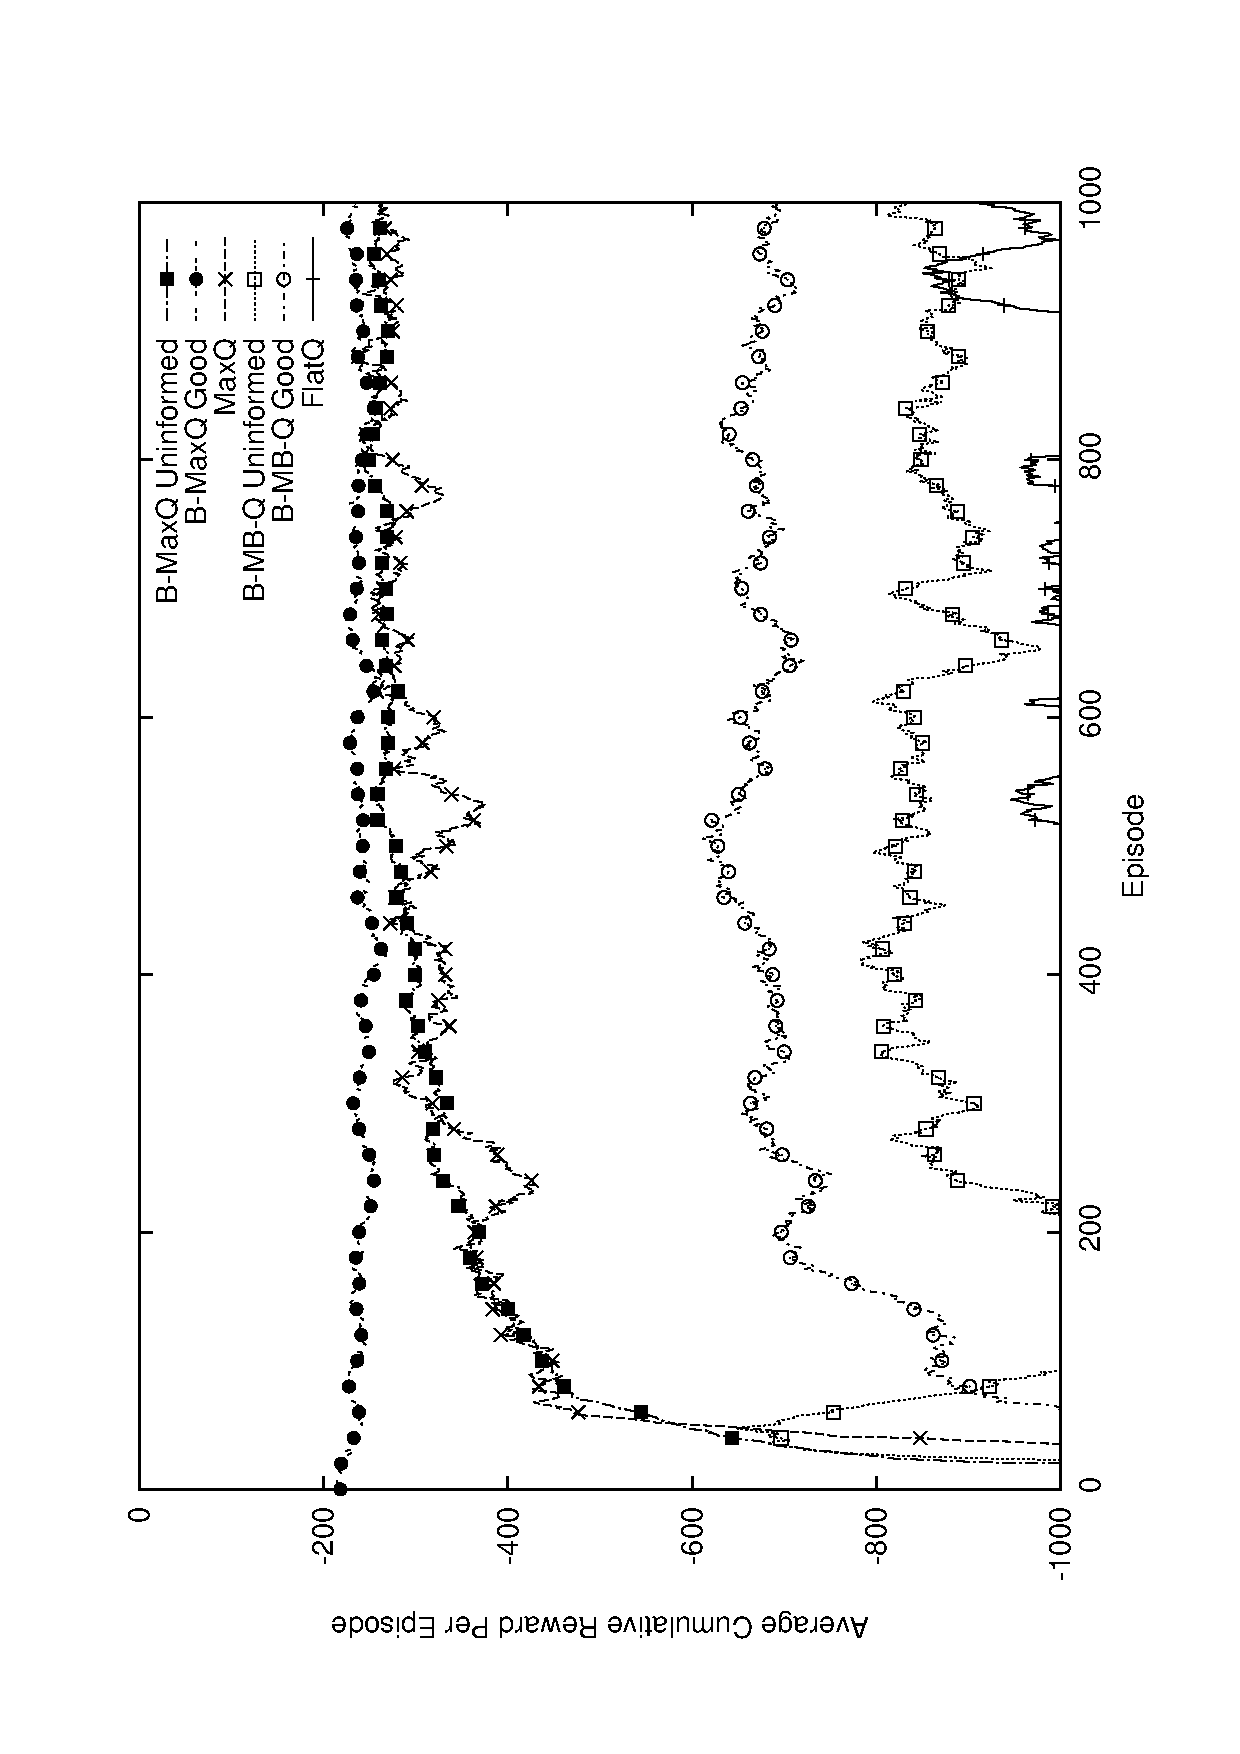
\includegraphics[scale=0.4]{Wargus3322.pdf}}
\vspace{-0.5in}
\caption{Performance of different algorithms on {\sf
    Resource-collection}.  The
  prefix ``B-'' denotes Bayesian, ``Uninformed/Good'' denotes the
  prior and ``MB'' denotes model-based.}\label{fig:rc}
\end{figure*}

To evaluate these hypotheses, we use two domains, two prior
distributions and a number of baseline methods. The two domains we use
are the well-known {\sf Taxi-world}~\cite{d-hrl-00} and {\sf
  Resource-collection}~\cite{mehta.icml08}. In {\sf Taxi-world}, the agent
controls a taxi in a grid-world that has to pick up a passenger from a
source location and drop them off at their destination. The state
variables consist of the location of the taxi and the source and
destination of the passenger. The actions available to the agent
consist of navigation actions and actions to pickup and putdown the
passenger.  The agent gets a reward of +20 upon completing the task, a
constant -1 reward for every action and a -10 penalty for an erroneous
action (e.g. trying to putdown a passenger when it is not carrying
one). We use a more challenging variant of this basic task, the
``fickle taxi'', where each navigation action has a 15\% chance of
moving in a direction orthogonal to the intended move (so 30\% chance
total). The {\sf Resource-collection} domain is inspired by real-time
strategy games where one component involves collecting resources from
a map in order to build units. We simulate this through a grid world
environment where the agent controls a unit that can harvest gold and
chop wood. Here the state variables consist of the location of the
agent, what the agent is carrying, whether a goldmine or forest is
adjacent to its current location and whether a desired gold or wood
quota has been met. The actions available to the agent are to move
to a specific location, chop gold or harvest wood, and to deposit the item it is
carrying (if any). To make the task tractable we limit the set of
possible moves to a set of four locations adjacent to each goldmine, forest
or deposit location. As before, for each navigation action the agent has
a probability of successfully completing it with 0.7 probability and
moving to a random location with 0.3 probability. Further, in this
domain, there may be multiple goldmines and multiple forests and
multiple locations next to each goldmine and forest, so the action
space is still quite large. In our experiments, the map contains two
goldmines and two forests, each containing two units of gold and two
units of wood, and the gold and wood quota is set to three each. The
agent gets a +50 reward when it meets the gold/wood quota, a constant -1
reward for every action and an additional -1 if it takes a ``bad''
action (such as trying to deposit when it is not carrying anything).
The task hierarchies corresponding to these domains are shown in
Figure~\ref{fig:tasks}.

For each domain, for the Bayesian methods, we use Dirichlet priors for
the transition function parameters and Normal-Gamma priors for the
reward function parameters. We use two different parameter settings for these
priors. The first case is an uninformed prior. Here the priors
 are set to approximate a uniform distribution over model
parameters. The second case is a ``good'' prior. In this case, we
first run the Bayesian MAXQ approach for 1000 episodes on each
problem, and use the estimated model posterior as the prior. The prior
distributions we choose are conjugate to the likelihood, so we can compute the
posterior distributions over the relevant parameters in closed form.
In general, this is not necessary; more complex priors could be used
as long as we can sample from the posterior distribution.

The methods we use in our experiments are: (i) Flat Q, the standard,
non-Bayesian Q-learning algorithm, (ii) MAXQ-0, the standard,
non-Bayesian Q-learning algorithm for MAXQ with no pseudo-reward,
(iii) Bayesian model-based Q-learning with uninformed prior and (iv) with
a ``good'' prior, (v) Bayesian MAXQ (our proposed approach) with a
uninformed and (vi) with a ``good prior.'' In our implementation, the
Bayesian model-based Q-learning uses the same code as the Bayesian
MAXQ algorithm, with a ``trivial'' hierarchy consisting of the Root
task with only the primitive actions as children. We make two changes
to the Bayesian MAXQ algorithm for efficiency: first, we use ``all
states updating''~\cite{d-hrl-00}, where the completion function is
updated fro all states seen in the child task rather than just the
exit. Second, in
Line~\ref{line:sample} in {\sc Recompute\_value}, we sample a model
from the posterior~\cite{Strens}. We observed that, as noted by
others~\cite{icml2007}, the convergence behavior can be improved by
sampling an approximately MAP model. We
approximate this by computing the MAP model from our posterior, and
then using an $\epsilon$-greedy hierarchical policy to select
actions. The results of these experiments are shown in
Figures~\ref{fig:taxi} and~\ref{fig:rc}. For the Bayesian methods, the
update frequency $k$ was set to 50 for {\sf Taxi-world} and 25 for
{\sf Resource-collection}. $Sim$ was set to 200 for Bayesian MAXQ for
{\sf Taxi-World} and 1000 for Bayesian model-based Q, and to 1000 for
both for {\sf Resource collection}.

From these results, comparing the Bayesian versions of MAXQ to the
non-Bayesian version, we observe that for {\sf Taxi-world}, the
Bayesian version converges faster to the optimal policy even with the
uninformed prior, while for {\sf Resource-collection}, the convergence
rates are similar. When a good prior is available, convergence is
very fast (almost immediate) in both domains. Thus, the availability
of model priors can help speed up convergence in many cases, even for HRL.

Next, we compare the Bayesian MAXQ approach to the ``flat'' Bayesian
model-based Q learning (which is nearly identical except the lack of
the task hierarchy). We note that in {\sf Taxi-world}, with uninformed
priors, though the ``flat'' method initially does worse, it soon catches up to standard
MAXQ and then to Bayesian MAXQ. This is probably because in this
domain, the primitive models are relatively easy to acquire, and the
task hierarchy provides no additional leverage. Note that for the
``good'' prior in this task, Bayesian MAXQ and flat Bayesian
model-based learning do about equally well. This indicates that in some
cases the availability of a good model prior may reduce the need for a
task hierarchy. However, this does not always happen, as shown in the
{\sf Resource-collection} domain, where even with a good prior,
``flat'' Bayesian model-based Q does not converge. The difference is
that in this case, the task hierarchy encodes extra information that
cannot be deduced just from the models. In particular, the task
hierarchy tells the agent that good policies consist of gold/wood
collection moves followed by deposit moves. Since the reward structure
in this domain is very sparse, it is difficult to deduce this even if very
good models are available. Thus, good priors may not be sufficient to
guarantee fast convergence---task hierarchies can encode additional
information about good policies that help convergence even in the presence
of good priors. However, if no such policy information is encoded by
the hierarchy (e.g. the hierarchy allows all ``legal'' policies),
then a good prior on the model reduces or eliminates the convergence advantage of
HRL over flat RL.

Finally, we compare the time taken by the different approaches in our
experiments in {\sf Taxi-world} (Table~\ref{tab:time}). We observe that, as expected, the
Bayesian RL approaches are significantly slower than the non-Bayesian
approaches. However, out of the Bayesian methods, the Bayesian MAXQ approaches are
significantly faster than the flat Bayesian model-based
approaches. This can be attributed to the fact that for the flat case,
during the simulation in {\sc Recompute\_value}, a much larger task
needs to be solved, while the Bayesian MAXQ approach is able to take
into account the structure of the hierarchy to only simulate subtasks
as needed, which ends up being much more efficient. However, we note
that we allowed the flat Bayesian model-based approach 1000 episodes
of simulation as opposed to 200 for Bayesian MAXQ. Clearly this
increases the time taken for the flat cases. But at the same time,
this is necessary: the ``Comparable Simulations'' row (and curve in
Figure~\ref{fig:taxi}) shows that, if the simulations are reduced to
250 episodes for this approach, the resulting values are no longer reliable and the performance of
the Bayesian flat approach drops sharply. Thus, taking advantage of
the hierarchical task decomposition helps reduce the computational cost of
Bayesian RL.

\label{sec:expts}
\begin{table*}[t]
\caption{CPU time taken by various methods on {\sf Taxi-world}.}
\label{tab:time}
\begin{center}
\begin{tabular}{| p{4cm} | l | l | l | l | l |}
\hline
\multirow{5}{*}{Method} 	&Tot. Time  for	&\multicolumn{2}{|c|}{}  &\multicolumn{2}{|c|}{}			\\ 
						&500 Episodes 	&\multicolumn{2}{|c|}{Episodes with} 	 &\multicolumn{2}{|c|}{Episodes with}			\\
						&(s)				&\multicolumn{2}{|c|}{5-20 Steps}	&\multicolumn{2}{|c|}{70-120 Steps} 		\\ 
						&				&\multicolumn{2}{|c|}{(near-optimal)}		&\multicolumn{2}{|c|}{(suboptimal)}				\\ \cline{3-6}
						&
                                                &Avg Time (ms)	&Count
                                                &Avg Time (ms)	&Count \\ \hline
						
Bayesian MaxQ, Uninformed Prior	&179	&21		&81 		&332  	&39 				\\ \hline
Bayesian Model-based Q, Uninformed Prior	&232	&162 	&211 	&851	&25 					\\ \hline
Bayesian MaxQ, Good Prior		&14		&17 		&209 	&84 		&3 				\\ \hline
Bayesian Model-based Q, Good Prior		&119	&172 	&316 	&- 		&0 				\\ \hline
Bayesian Model-based Q, Good Prior \& Comparable Simulations 									&934	&- 		&0		&687	&56		\\ \hline
MaxQ							&0.53	&- 		&0		&1.49 	&171				\\ \hline
Flat Q							&1.15	&- 		&0		&0.37	&18			\\ \hline
\end{tabular}
\end{center}
\end{table*}
